\documentclass{beamer}

\usepackage{amsmath}
\usetheme{Marburg} 
\usepackage{graphicx}
\usepackage{color,listings}

\DeclareGraphicsExtensions{.png}


\lstset{language=java}
\lstset{breaklines=true}
\lstset{showstringspaces=false}
\lstset{tabsize=3}
\lstset{basicstyle=\ttfamily\scriptsize}
\lstset{breakautoindent=true}
\lstset{postbreak=\space}
\title{An Eclipse-based Integrated and Automated
Fault Localization System}
\author{Tristan Challener}
\date{\today}

\begin{document}
	\begin{frame}
	\titlepage
	\end{frame}
	
	%%%%%%%%%%%% Slide %%%%%%%%%%%%%%%%%%%%%%%%%%%%%%%%%%%%%%%%%%%%%%%%%%%
	\section{Contents}
	\begin{frame}
	\frametitle{Table of Contents}
	\begin{enumerate}
	  \item Motivation
	  \item External Components
	    \begin{enumerate}
	      \item Automatic Fault Localization
	      \item Per-Test Coverage
	      \item Mutation
	    \end{enumerate}
	  \item Implementation
	    \begin{enumerate}
	      \item Parsing Containers
	      \item Intermediate Representation
	      \item Final Representation
	      \item System Output
	    \end{enumerate}
	  \item Experiment
	  	\begin{enumerate}
	  	  \item Case Application
	  	  \item Mutant Insertion
	  	  \item Results Analysis
	  	\end{enumerate}
	  \item Conclusion
	\end{enumerate}
	\end{frame}
	%%%%%%%%%%%% Slide %%%%%%%%%%%%%%%%%%%%%%%%%%%%%%%%%%%%%%%%%%%%%%%%%%%
	\section{Motivation}
	\begin{frame}
	\frametitle{Motivation}
	\begin{itemize}
	  \item Debugging is complex and difficult
	    \pause
	  \item Fault localization is the most expensive
	    \pause
	  \item Current techniques can be improved
	\end{itemize}
	\end{frame}
	%%%%%%%%%%%% Slide %%%%%%%%%%%%%%%%%%%%%%%%%%%%%%%%%%%%%%%%%%%%%%%%%%%
	\section{Components}
	\subsection{AFL}
	\begin{frame}
	\frametitle{Automatic Fault Localization}
	\begin{itemize}
	  \item Uses per-test coverage analysis
	    \pause
	  \item Ranks statements by suspiciousness
	    \pause
	  \item Variety of risk evaluation functions\\
	  	Tarantula equation:
	  \begin{equation}
	suspiciousness(e) = 1 - \frac{\frac{failed(e)}{total failed}}{\frac{passed(e)}{total passed} + \frac{failed(e)}{total failed}}
	  \end{equation}
	\end{itemize}
	\end{frame}
	%%%%%%%%%%%% Slide %%%%%%%%%%%%%%%%%%%%%%%%%%%%%%%%%%%%%%%%%%%%%%%%%%%
	\subsection{Coverage}
	\begin{frame}
	\frametitle{CodeCover Coverage}
	\begin{itemize}
    	\item Eclipse-compatible coverage analysis tool
    	\pause
    	\item Uses existing JUnit test suites
    	\pause
    	\item Generates coverage information for each test method
    	\pause
    	\item Stores output in readable format (XML)
	\end{itemize}
	\end{frame}
	%%%%%%%%%%%% Slide %%%%%%%%%%%%%%%%%%%%%%%%%%%%%%%%%%%%%%%%%%%%%%%%%%%
	\begin{frame}
	\frametitle{CodeCover}
	  	\begin{figure}
	  		\label{coverage}
	  		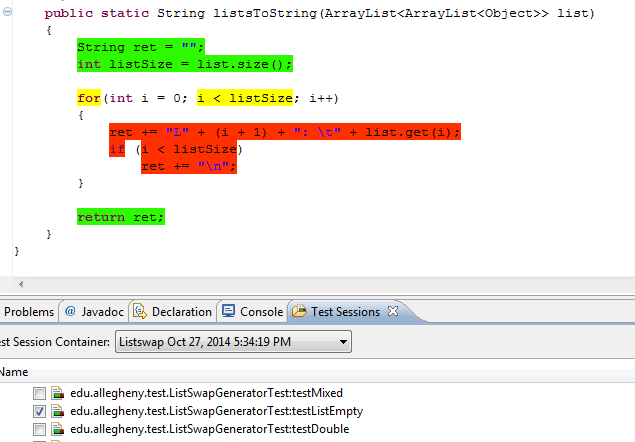
\includegraphics[width=4in]{img/codecovercoverage}
	  	\end{figure}
	\end{frame}
	%%%%%%%%%%%% Slide %%%%%%%%%%%%%%%%%%%%%%%%%%%%%%%%%%%%%%%%%%%%%%%%%%%
	\subsection{Mutation}
	\begin{frame}
	\frametitle{MAJOR Mutation}
	\begin{itemize}
		\item Introducing faults for experimental evaluation
		\pause
		\item MAJOR mutation system
		\pause
		\item Representative of real-world faults
	\end{itemize}
	\end{frame}
	%%%%%%%%%%%% Slide %%%%%%%%%%%%%%%%%%%%%%%%%%%%%%%%%%%%%%%%%%%%%%%%%%%
	\section{Implementation}
	\subsection{Parsing Containers}
	\begin{frame}
	\frametitle{Parsing XML}
	\begin{itemize}
		\item CodeCover stores information as XML
		\pause
		\item Parse using Java DOM
		\pause
    	\item Contains several pieces of information:
    	\pause
    	\begin{itemize}
    		\item Complete source code
    		\item Statement definitions
    		\item List of statements covered by each test method for each file under test
    		\pause
    	\end{itemize}
	\end{itemize}
	\begin{figure}
		\label{xmlstat}
		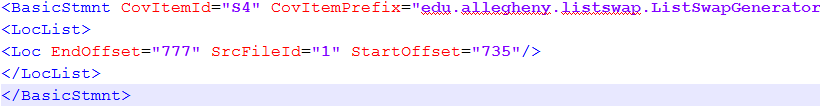
\includegraphics[width=4in]{img/xmlstatement}
	\end{figure}
	\end{frame}	
	%%%%%%%%%%%% Slide %%%%%%%%%%%%%%%%%%%%%%%%%%%%%%%%%%%%%%%%%%%%%%%%%%%
	\begin{frame}
	\frametitle{Coverage}
	  	\begin{figure}
	  		\label{xmlcov}
	  		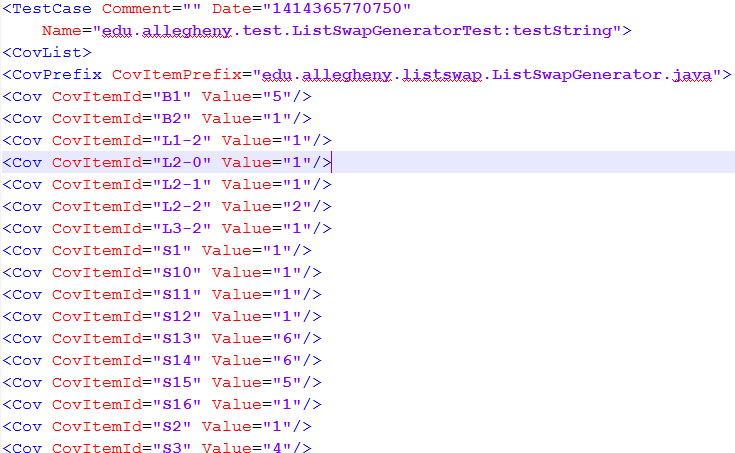
\includegraphics[width=4in]{img/xmlcoverage}
	  	\end{figure}
	\end{frame}
	%%%%%%%%%%%% Slide %%%%%%%%%%%%%%%%%%%%%%%%%%%%%%%%%%%%%%%%%%%%%%%%%%%
	\subsection{Intermediate Representation}
	\begin{frame}
	\frametitle{Intermediate Representation}
	\begin{itemize}
		\item DOM is overly complex for multi-pass analysis\
		\pause
		\item Store information in a more accessible form
		\pause
	\end{itemize}
	
	\begin{figure}
		\label{ir}
		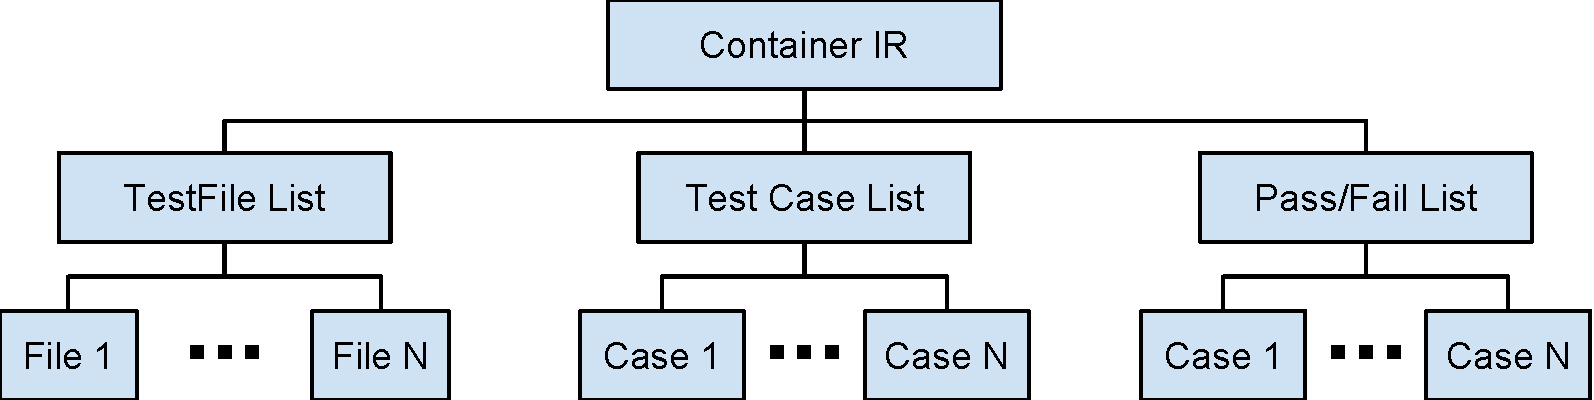
\includegraphics[width=4in]{img/ContainerIR.pdf}
	\end{figure}
	
	\end{frame}
	%%%%%%%%%%%% Slide %%%%%%%%%%%%%%%%%%%%%%%%%%%%%%%%%%%%%%%%%%%%%%%%%%%
	\subsection{Final Representation}
	\begin{frame}
	\frametitle{Final Representation}
	\begin{itemize}
		\item IR is still not conducive to risk evaluation
		\pause
		\item Reformat information into a simpler representation
		\pause
		\item Designed to allow very simple suspiciousness analysis
		\pause
	\end{itemize}
	
	\begin{figure}
		\label{sr}
		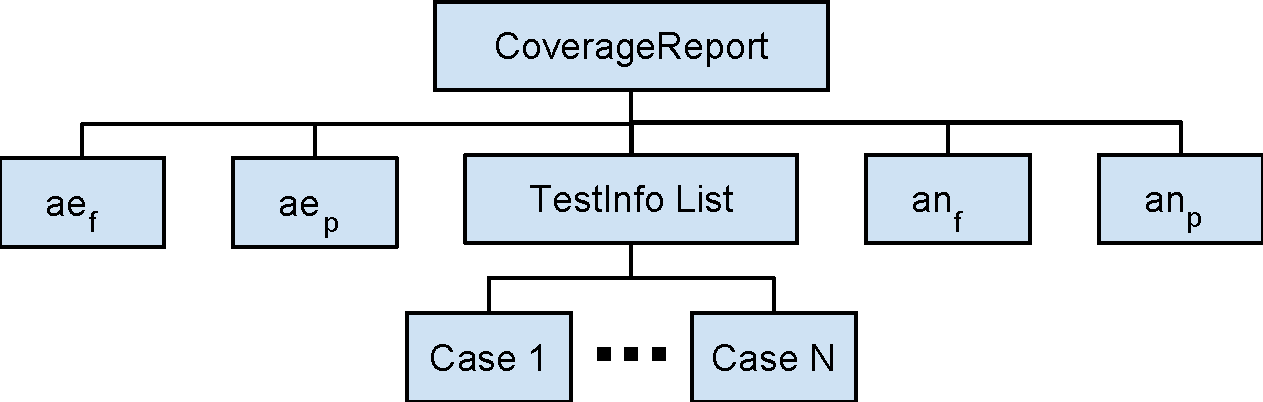
\includegraphics[width=4in]{img/CoverageReport.pdf}
	\end{figure}
	\end{frame}
	%%%%%%%%%%%% Slide %%%%%%%%%%%%%%%%%%%%%%%%%%%%%%%%%%%%%%%%%%%%%%%%%%%
	\subsection{System Output}
	\begin{frame}
	\frametitle{System Output}
	\begin{itemize}
		\item Output data in CSV format
		\pause
		\item Conform to Tidy Data standard
		\pause
	\end{itemize}
	
	\begin{figure}
		\label{out}
		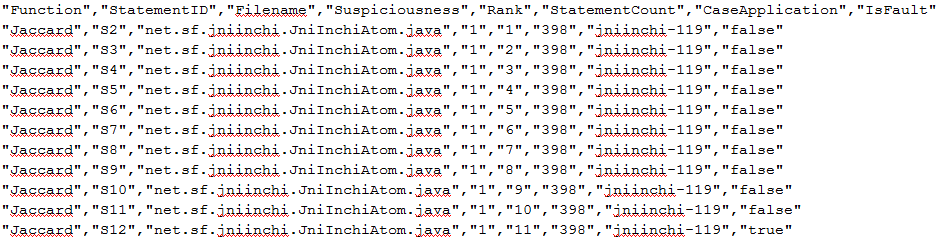
\includegraphics[width=4in]{img/output}
	\end{figure}
	
	\end{frame}
	%%%%%%%%%%%% Slide %%%%%%%%%%%%%%%%%%%%%%%%%%%%%%%%%%%%%%%%%%%%%%%%%%%
	\section{Experiment}
	\subsection{Case Application}
	\begin{frame}
	\frametitle{Case Application}
	\begin{itemize}
		\item Obtained case applications from Sarojini Balasubramanian
		\pause
		\item Several applications prepared for use with MAJOR
		\pause
		\item Only one (Jni-InChi) could be processed by CodeCover
	\end{itemize}
	\end{frame}
	%%%%%%%%%%%% Slide %%%%%%%%%%%%%%%%%%%%%%%%%%%%%%%%%%%%%%%%%%%%%%%%%%%
	\subsection{Mutant Insertion}
	\begin{frame}
	\frametitle{Mutant Insertion}
	\begin{itemize}
		\item Faults must be introduced for experimentation
		\pause
		\item MAJOR analysis information provided by Sarojini
		\pause
		\item Killed mutants of various types selected and inserted into Jni-InChi
	\end{itemize}
	
	\begin{figure}
		\label{mutants}
		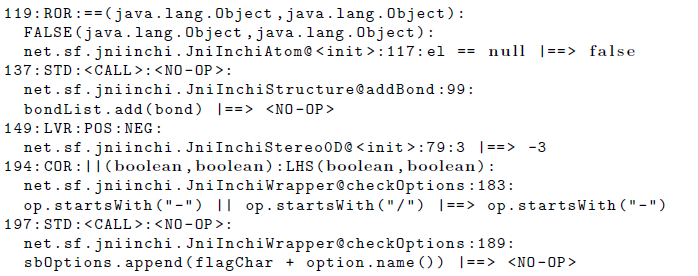
\includegraphics[width=4in]{img/mutants}
	\end{figure}
	
	\end{frame}
	%%%%%%%%%%%% Slide %%%%%%%%%%%%%%%%%%%%%%%%%%%%%%%%%%%%%%%%%%%%%%%%%%%
	\subsection{Results Analysis}
	\begin{frame}
	\frametitle{Results Analysis}
	\begin{itemize}
		\item System executed on the CodeCover output for five mutants of Jni-Inchi
		\pause
		\item CSV Output imported into R
		\pause
		\item Plots generated for individual mutants and average overall
	\end{itemize}
	
	\begin{figure}
		\label{r}
		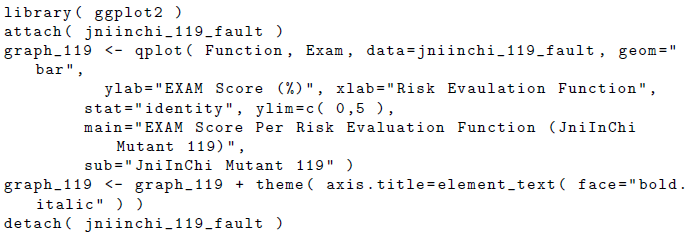
\includegraphics[width=4in]{img/ggplot}
	\end{figure}
	\end{frame}
	%%%%%%%%%%%% Slide %%%%%%%%%%%%%%%%%%%%%%%%%%%%%%%%%%%%%%%%%%%%%%%%%%%
	\begin{frame}
	\frametitle{Results}
	\begin{figure}
		\label{results}
		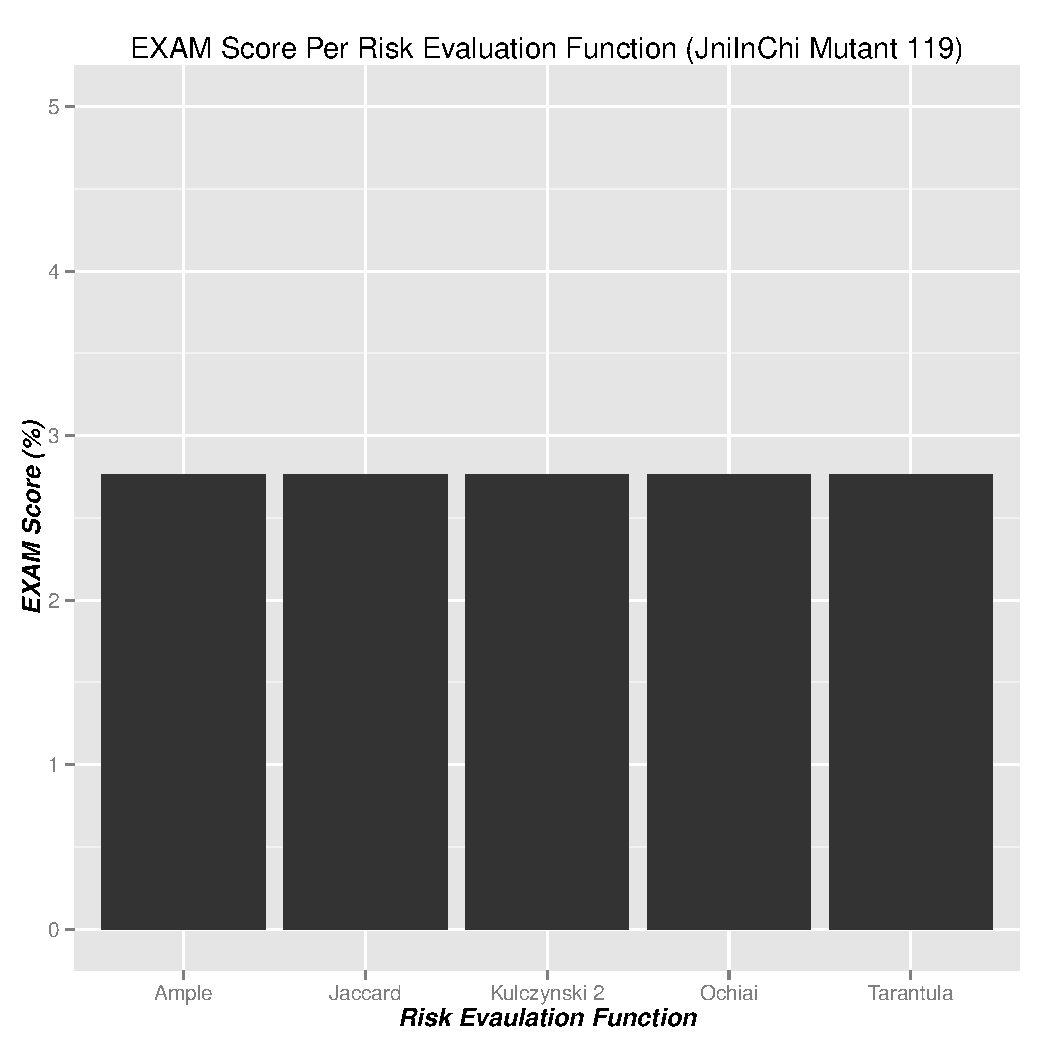
\includegraphics[width=1.8in]{img/graph_119.pdf}
		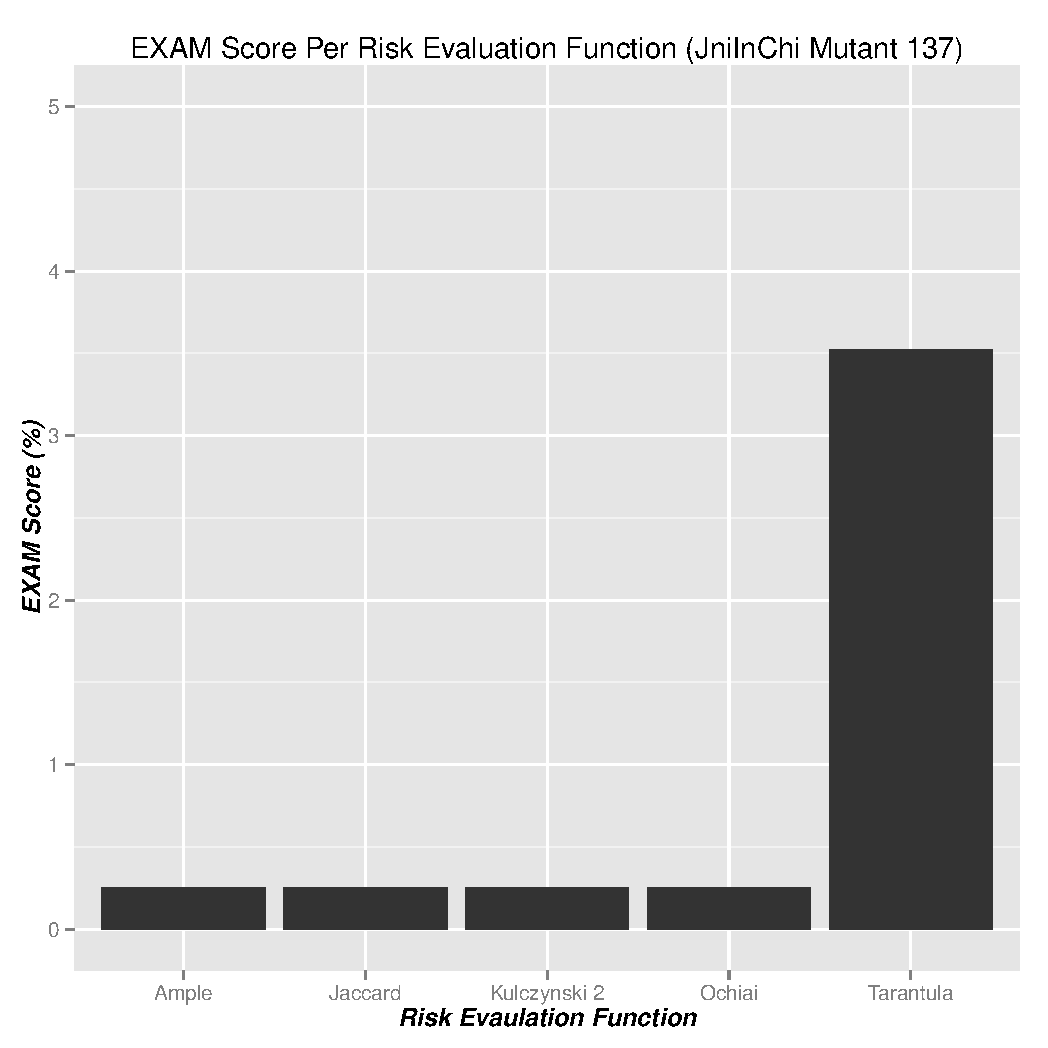
\includegraphics[width=1.8in]{img/graph_137.pdf}
	\end{figure}
	\end{frame}
	%%%%%%%%%%%% Slide %%%%%%%%%%%%%%%%%%%%%%%%%%%%%%%%%%%%%%%%%%%%%%%%%%%
	\begin{frame}
	\frametitle{Results}
	\begin{figure}
		\label{results}
		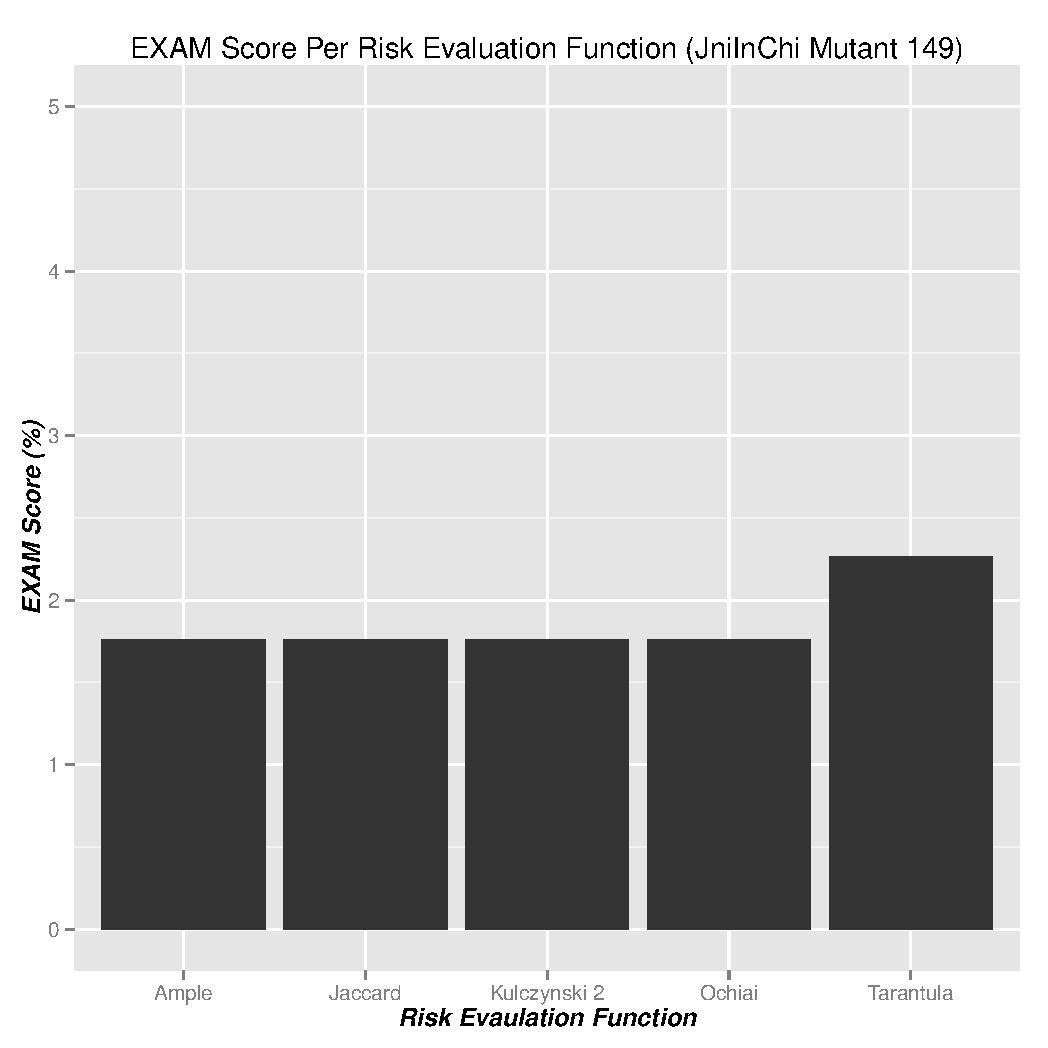
\includegraphics[width=1.8in]{img/graph_149.pdf}
		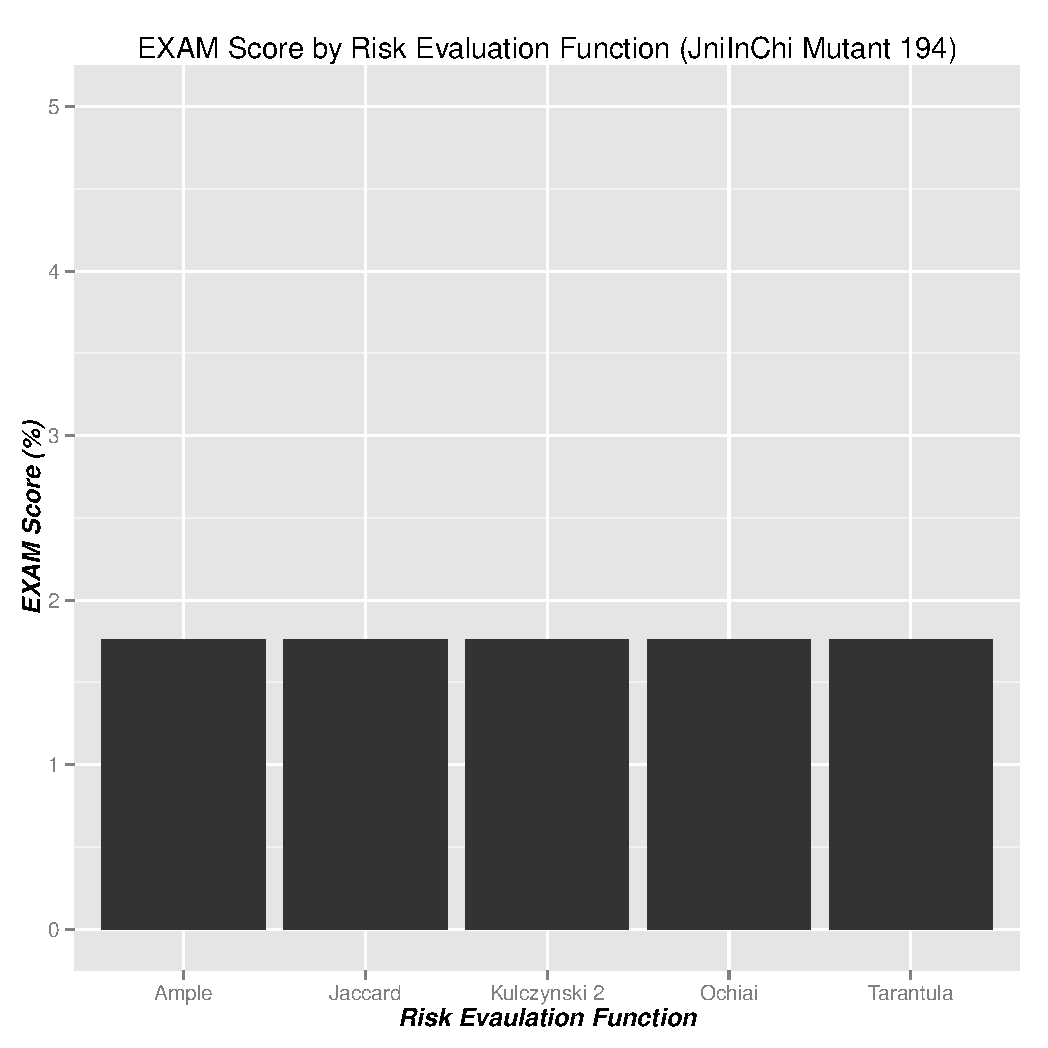
\includegraphics[width=1.8in]{img/graph_194.pdf}
	\end{figure}
	\end{frame}
	%%%%%%%%%%%% Slide %%%%%%%%%%%%%%%%%%%%%%%%%%%%%%%%%%%%%%%%%%%%%%%%%%%
	\begin{frame}
	\frametitle{Results}
	\begin{figure}
		\label{results}
		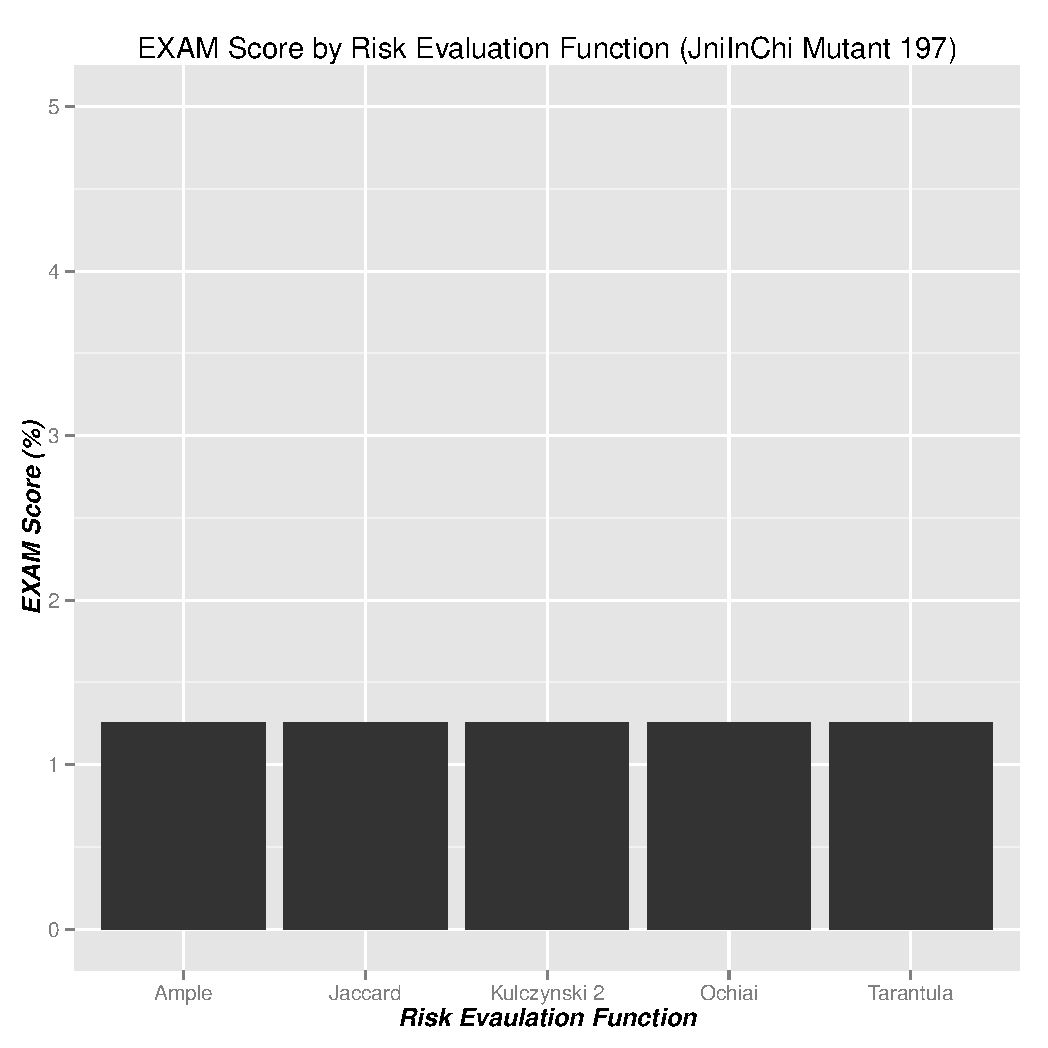
\includegraphics[width=1.8in]{img/graph_197.pdf}
		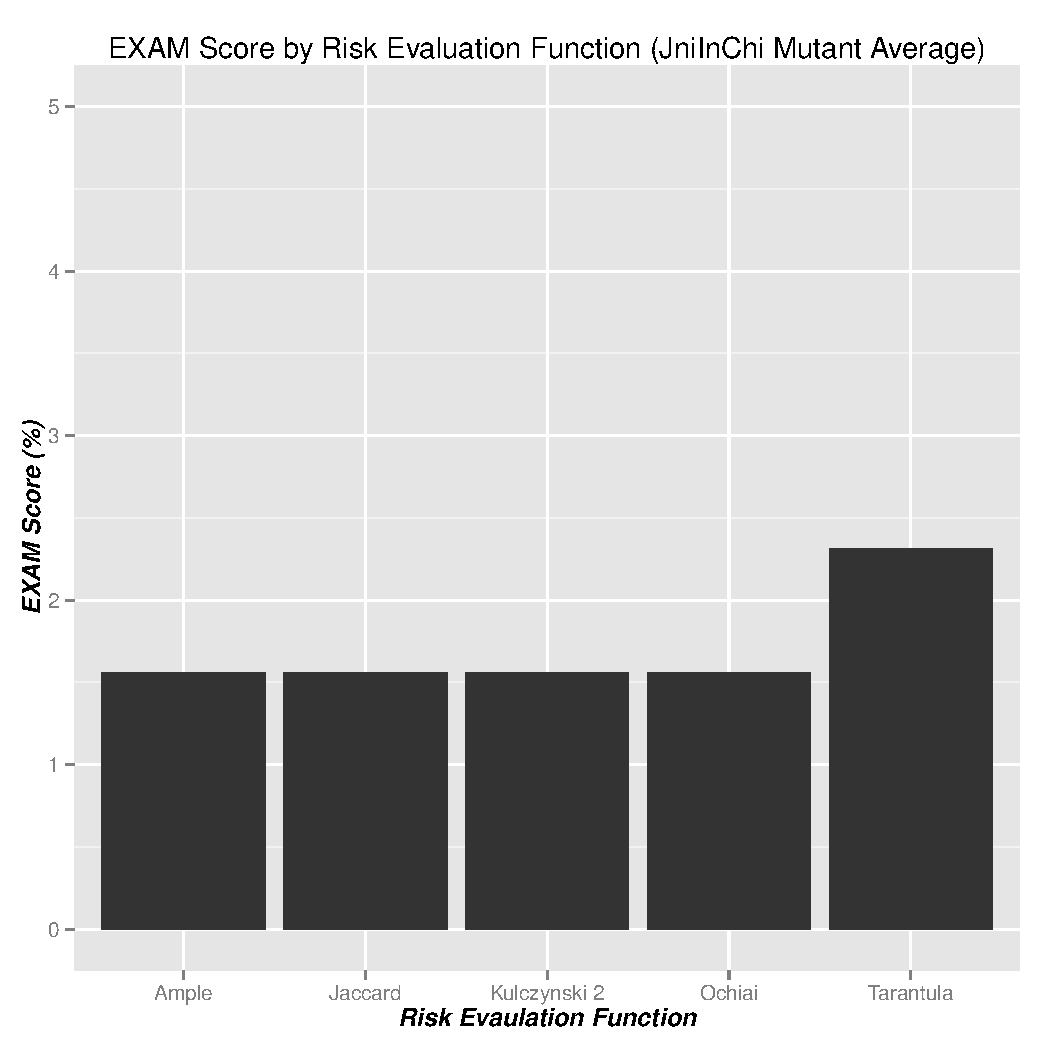
\includegraphics[width=1.8in]{img/graph_avg.pdf}
	\end{figure}
	\end{frame}
	%%%%%%%%%%%% Slide %%%%%%%%%%%%%%%%%%%%%%%%%%%%%%%%%%%%%%%%%%%%%%%%%%%
	\section{Conclusion}
	\begin{frame}
		\frametitle{Conclusion}
		\begin{itemize}
	    	\item Of our two original goals, the first proved infeasible
	    	\pause
	    	\item Implemented a system to apply suspiciousness evaluation to coverage data
	    	\pause
	    	\item Completed a small study
	    	\pause
	    	\item No statistically significant results generated due to CodeCover limitations
			\pause
			\item Several possible areas for future work identified
		\end{itemize}
	\end{frame}
\end{document}
